\documentclass{article}
\usepackage[utf8]{inputenc}
\usepackage{graphicx}
\usepackage{verbatim}
\usepackage{rotating}
\usepackage{color}
\usepackage{a4}
\title{320 Requirements}
\author{Trevor's Team}
\date{\today}

\begin{document}
\begin{titlepage}

\maketitle
\begin{abstract}
\textbf{Purpose of System:} \newline
\newline
The purpose of this system is to be an online tutor for students at the University of Massachusetts Amherst. This learning tool would help teach the students and allow them to create ER diagrams and submit them as homework assignments. They can then be graded by solutions uploaded by the instructor of a course. Feedback will then be provided to help the student learn from their mistakes. The benefits of this system is that it makes submitting learning in the course and submitting homework much easier for both the students and instructor. \newline
\textbf{Scope:}
\newline \newline
This document will clearly outline the requirements and the system requirements of ER Diagram Tutoring System. This document should cover all key concepts and fundamental requirements. The requirements should satisfy the standards of the client and provide accuracy in the functionality of the system. 


\end{abstract}
\end{titlepage}
\tableofcontents
\newpage


\chapter{Data Dictionary}

\vspace{1.5cm}
\begin{table}[H]

\scalebox{0.6}{
    \begin{tabular}{ | l | l | l |l| p{5cm} |}
  \hline
    Student Info & Instructor Info & Author Info & Retrieve Question \\ \hline


    - student ID	&  - instructor ID  &  - author ID          & - question ID  \\
    - password		&  - password      	&  - password           & - question  \\ 
					&              	  	&                       & - assignment ID\\ \hline

    
       
    
Submit Answer		  	& Send Student Score & Send Feedback 				& Display Class Info\\ \hline

       - student ID   	&  - student ID    	 &  - question ID				& - class ID  \\ 
       - question ID  	&  - instructor ID   &  - feedback information      & \\
	   - student answer &  - student score   &               				&\\ \hline
    
    
Display Feedback		  	& Class Info 		& Update Question 				& Create New Questions/Answers\\ \hline

       - student ID   			&  - student ID   		 &  - question ID				& - question ID  \\ 
       - student answer 		&  					  	 &  - question info			    & - question info\\
	   - question ID 			&  					   	 &               				& - answer(s) info\\ \hline    
    
    
Check Scores		  	& Check Answers 		& Update Scores 				& \\ \hline

       - student ID 			&  - question ID   		 &  - student ID				&   \\ 
       - question ID 			&  - student ID		  	 &  - question ID		   		&  \\
								&  - student answer	  	 &  - student answer		    &  \\	   
	    						&  - question answer  	 &               				&  \\ \hline       
    
    
    
    \hline
   
    \end{tabular}
    }
 \caption{Data Dictionary}
\end{table}

    

    




\newpage

\iffalse
\begin{section}{Context Level Diagram}
    \begin{figure}[h!]
        \begin{center}
          \centerline{ 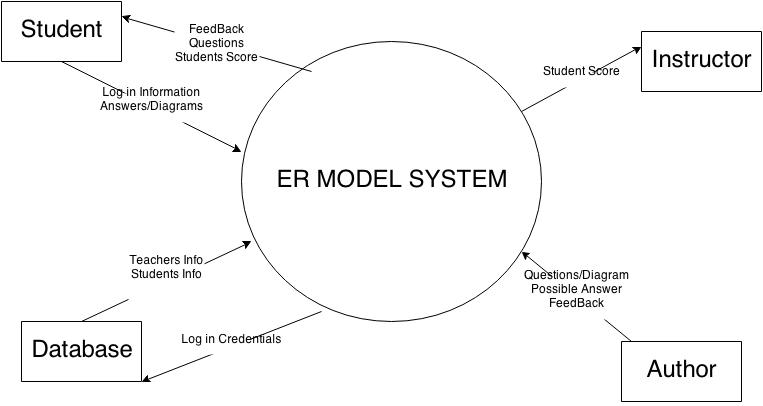
\includegraphics[height=13cm]{Context Diagram.jpg}}
            \caption{DFD Context Diagram}
        \end{center}
    \end{figure}
\end{section}
\newpage
\begin{section}{Level 0 Diagram}
    \begin{figure}[h!]
        \begin{center}
            \centerline{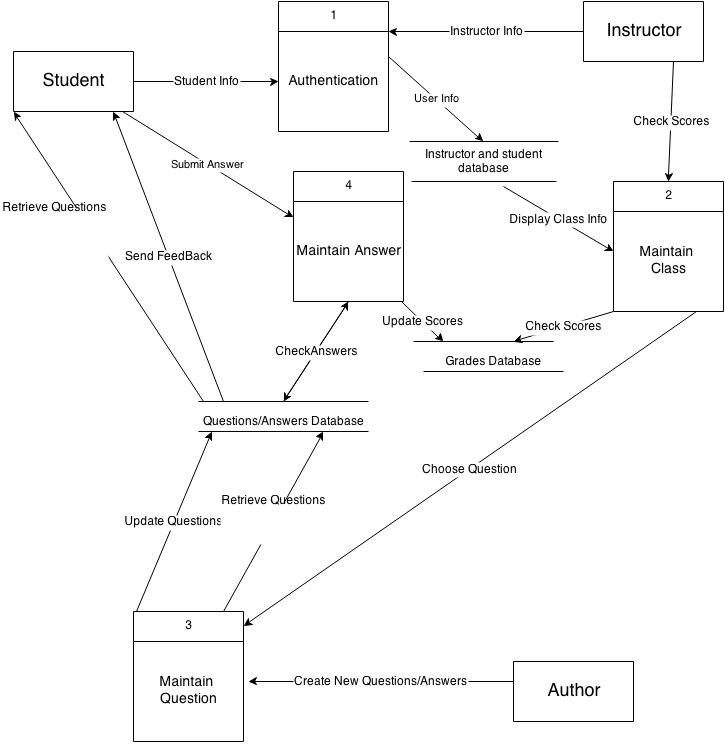
\includegraphics[height=13cm]{DFD Level 0.jpg}}
            \caption{DFD Level 0 Diagram}
        \end{center}
    \end{figure}
\end{section}
\newpage
\fi


    \chapter{Functional Requirements}
%\section{Functional Requirements}
    \begin{section}{Allow Student to Draw a Diagram}
        Description: Student given tools and space to draw an ER diagram \newline
        Primary Actor: Student \newline
        Precondition: Student is logged in and viewing a            question \newline
        Trigger: Student chooses a question to work on \newline
        Success end condition: Student can submit answer            \newline
        Failed end condition: Diagram is not drawn \newline
        \newline
        Steps:
        \begin{enumerate}
            \item{Empty space available to draw diagram}
            \item{Student picks a diagram type (Chen’s/Crow’s Foot)}
            \item{Student picks shapes from toolbox and places in           diagram}
            \item{Student places text inside shapes}
            \item{Student places links between shapes}
            \item{Student can edit or remove anything already placed on the diagram before finalizing}
        \end{enumerate}
        Exceptions:
        \begin{itemize}
            \item{Teacher draws diagram that students must edit             \newline
                *Draw space will not be empty, student will be able to           make changes to present diagram}
        \end{itemize}
    \end{section}

    
    \begin{section}{Submit Answer}
        Description: Student submits answer to be checked and saved by the system \newline
        Primary Actor:Student \newline
        Precondition: Student is ready to submit answer \newline
        Trigger: Pressing the submit button \newline
        Success end condition: Feedback and/or grade is given       \newline
        Failed end condition: Nothing is given back to student      \newline
        \newline
        Steps:
        \begin{enumerate}
            \item{Student submits answer by pressing the submit             button}
            \item{System processes answer and decides validity}
            \item{Outputs feedback and/or grade for student to see}
            \item{Answer is saved into database}
        \end{enumerate}
        Exceptions:
        \begin{itemize}
            \item{Student leaves area blank \newline
        	*Answer is just marked as wrong}
            \item{Author never properly input the correct answer or     feedback \newline
        	*Student is told that there's nothing to report}
        \end{itemize}
    \end{section}

    
    \begin{section}{Allow Teacher to Create    Questions/Feedback}
        Description: Teacher creates a question and adds it to a specific assignment \newline
        Primary Actor: Teacher \newline
        Precondition: Teacher is logged in a specific course. \newline
        Trigger: Teacher selects a specific Homework to create a     question. \newline
        Success end condition: Question is uploaded and the instructor is able to see it. \newline
        Failed end condition: Students don’t see the question       properly. \newline
        \newline
        Steps:
        \begin{enumerate}
            \item{Teacher clicks on a “create” button to create the           question.}
            \item{Teacher select the number of the question that             he/she wants to post for a previously chosen               homework.}
            \item{Teacher writes the database schema of the ER              diagram that is going to be drawn by the student, in         an available textbox.}
            \item{Teacher provides a general feedback in a textbox            provided.}
            \item{Teacher clicks on a “add” button to add the                 question of the homework.}
            \item{Teacher clicks on a “preview” button to see the           students point of view of the entire homework.}
            \item{Teacher clicks on a “submit” button to submit the           entire homework.}
        \end{enumerate}
        Exceptions:
        \begin{itemize}
            \item{Teacher tries to create question but he/she doesn't have Internet connection.}
        \end{itemize}
    \end{section}

    
    \begin{section}{Select Question to Answer}
        Description: Student views a question that he would like to answer \newline
        Primary Actor: Student \newline
        Precondition: Student is logged in and is in an assignment         \newline
        Trigger: The student attempts to select a new question      to attempt to answer \newline
        Success End Condition: Question that the student selects     successfully loads \newline
        Failed End Condition: The question that is selected does     not load \newline
        \newline
        Steps:
        \begin{enumerate}
            \item{Student scrolls through the list of questions in the assignment.}
            \item{Student selects the question they would like to        answer from the list.}
            \item{Webpage for the selected question loads}
            \item{Student can read and answer question}
        \end{enumerate}
        Exceptions: None
    \end{section}
        
    \begin{section}{Student Logs In}
        Description: The student is logging in, in order to access the tutor system using their NetID and password. \newline
        Primary Actor: Student \newline
        Secondary Actor: System \newline
        Precondition: The student is on the login page of the system. \newline
        Trigger: The student wants to log into the tutoring system. \newline
        Successful End Condition: The student successfully logs into the tutoring system. \newline
        Failed End Condition:  The student is unable to log into the system because of an incorrect NetID or password or both \newline
        \newline
        Steps:
        \begin{enumerate}
            \item{The student enters their NetID in the username textbox}
            \item{The student enters their password in the password textbox}
            \item{The student clicks on the LOGIN button to enter the system}
        \end{enumerate}
        Exceptions:
        \begin{itemize}
            \item{If the student does not enter the correct NetID or password the system will 
            not log the student in and a message will appear stating that the NetID or password 
            that they entered is incorrect and to please try again.}
        \end{itemize}
    \end{section}
        
    \begin{section}{Student Views Assignments}
        Description: Once logged in, the student can view available assignments \newline
        Primary Actor: Student \newline
        Precondition: Student is already logged in \newline
        Trigger: Student logs in \newline
        Successful End Condition: Student can view all questions in an assignment \newline
        Failed End Condition: Student is unable to see any questions in the assignment \newline
        \newline
        Steps:
        \begin{enumerate}
            \item{Student clicks on desired assignment}
            \item{Student can select any of the question(s) in the assignment}
            \item{Student can go back to home page and select any other assignment}
        \end{enumerate}
        Exceptions:
        \begin{itemize}
            \item{There are no assignments available, student has nothing to view.}
        \end{itemize}
    \end{section}
    
    
    \begin{section}{Student Views Question}
        Description: The student views a question that is part of an assignment. \newline
        Primary Actor: Student \newline
        Secondary Actor: System \newline
        Precondition: The student is logged into the system. \newline
        Trigger: The student clicks on the question to view it. \newline
        Successful End Condition: The student views the question they have selected. \newline
        Failed End Condition: The student is unable to view the question. \newline
        \newline
        Steps:
        \begin{enumerate}
            \item{The student selects an assignment to view.}
            \item{The student then selects a specific question to view.}
            \item{The student views the question.}
        \end{enumerate}
        Exceptions: None
    \end{section}

    
    
    \begin{section}{Student Submits Answer to Question}
    
    
    
    \end{section
    
    \begin{section}{Student Views Feedback}
        Description: After submitting the question the student is able to see the feedback that is given for the 
        question based on if they answered the question correctly or not. \newline
        Primary Actor: Student \newline
        Secondary Actor: System \newline
        Precondition: The student has selected a question and answered the question. \newline
        Trigger: The student submits the answer to the question. \newline
        Successful End Condition: Feedback is displayed on the screen for the student 
        to read and use to help make their answer correct if it is incorrect. \newline
        Failed End Condition: There is no feedback that gets displayed. \newline
        \newline
        Steps:
        \begin{enumerate}
            \item{Once the answer has been submitted the system compares it to the correct answer given.}
            \item{If the answer is correct the question page displays the feedback that is 
            written by the author for a correct answer such as good job or correct.}
            \item{If the answer is incorrect the question page displays the feedback that is 
            written by the author for an incorrect answer such as a hint or common mistake.}
            \item{The student reads the feedback that is displayed on the screen.}
        \end{enumerate}
        Exceptions:
        \begin{itemize}
            \item{The author does not enter in any feedback for correct answers so no feedback will be displayed.}
            \item{The author does not enter in any feedback for incorrect answers so no feedback will be displayed.}
        \end{itemize}
    \end{section}
        
    \begin{section}{Author Logs In}
        Description: The author is logging in, in order to access the tutor system using their NetID and password. \newline
        Primary Actor: Author \newline
        Secondary Actor: System \newline
        Precondition: The author is on the login page of the system. \newline
        Trigger: The author wants to log into the tutoring system. \newline
        Successful End Condition: The author successfully logs into the tutoring system. \newline
        Failed End Condition:  The author is unable to log into the system because of an incorrect NetID or password or both \newline
        \newline
        Steps:
        \begin{enumerate}
            \item{The author enters his NetID in the username textbox}
            \item{The author enters his password in the password textbox}
            \item{The author clicks on the LOGIN button to enter the system}
        \end{enumerate}
        Exceptions:
        \begin{itemize}
            \item{If the author does not enter the correct NetID or password 
            the system will not log the student in and a message will appear stating 
            that the NetID or password that they entered is incorrect and to please try again.}
        \end{itemize}
    \end{section}
  
  
    
    \begin{section}{Author Views the Question Bank}
    
    \end{section}
    
    
    
    \begin{section}{Author Adds a New Question to Question Bank}
    
    \end{section}
    
    
    
    \begin{section}{Author Edits a Question From the Question Bank}
        Description: The author wants to edit a question that is already in the question bank by changing any or all of the different parts of the question. \newline
        Primary Actor: Author \newline
        Secondary Actor: System \newline
        Precondition: The author has already created the question that wish to edit. \newline
        Trigger: The author is viewing a question that they wish to edit. \newline
        Successful End Condition: The question changes have been made and the author is prompted that their changes have been made. \newline
        Failed End Condition: The question does not get updated and the author is prompted saying that the question was not changed. \newline
        \newline
        Steps:
        \begin{enumerate}
            \item{The author selects the edit button.}
            \item{The author edits the question text.}
            \item{The author edits the question correct answer.}
            \item{The author edits the question feedback.}
            \item{The author saves the changes to the question and answer.}
        \end{enumerate}
        Exceptions:
        \begin{itemize}
            \item{The author does not want to edit the question text so they do not edit it and leave it alone.}
            \item{The author does not want to edit the question correct answer so they do not edit it and leave it alone.}
            \item{The author does not want to edit the question feedback so they do not edit it and leave it alone.}
            \item{The author does not save the changes to the question so the changes are not saved.}
            \item{The author exits the system without saving the changes to the questions resulting in none of the changes being saved.}
        \end{itemize}
    \end{section}
    
    
    \begin{section}{Author Removes a Question From the Question Bank}
    
    \end{section}
    
    
    \begin{section}{Author Views a Question}
        Description: The author views questions that have been created. \newline
        Primary Actor: Author \newline
        Secondary Actor: System \newline
        Precondition: The author is logged into the system. \newline
        Trigger: The author has created a question and would like to view the question. \newline
        Successful End Condition: The author views the question that they would like to view. \newline
        Failed End Condition: The author is unable to view the question that they want to view. \newline
        \newline
        Steps:
        \begin{enumerate}
            \item{The author selects the questions tab from their view.}
            \item{The author then scrolls through the list of questions.}
            \item{The author then selects the question they would like to view.}
            \item{The author then views the question.}
        \end{enumerate}
        Exceptions: None
    \end{section}
    
    
    \begin{section}{Author Copies a Question} 
    
    \end{section}



\chapter{Environmental Requirements}


    \begin{section}{ToolBox for Drawing Diagram}
    A ToolBox will help the student and author draw the diagram. The user will first select whether he wants to draw a Chen's Diagram or a Crow's Foot Diagram. The toolbox will then adjust accordingly, displaying the shapes and edges that are common to the chosen diagram. This will include squares, circles, directed edges, and tick marks (for Crow's Foot).
    \end{section}
    
    \begin{section}{Save Progress of Current Assignment}
    When a student logs in, he/she should be able to start an assignment. As the student progresses through the assignment, the answers submitted by the student should be saved in the student's personal database. In that way, if he/she wants to stop and continue with the assignment another time, he/she can do so without starting all over again.
    \end{section}
    
    \begin{section}{List of Available Questions and Their Status}
    While a student is answering questions, there will be a list of all the questions in the current assignment listed horizontally at the top of the page.  Next to each question number will be a small image.  The image will either be a green check mark if the question is answered correctly, a red x is the question is answered incorrectly or a black question mark if the question has not been answered yet.  When the status of the question changes then so will the image next to the question number.
    \end{section}
    
    \begin{section}{Open Space to Draw Diagram}
    After a student selects which question they want to work on a white drawing space will be given to them in which to draw their answer. Off to the side of this space will be the toolbox which they use to do the drawing. There will also be a submit button off to the side somewhere which is what the student is to press when they're finished with their answer.
    \end{section}
    
    \begin{section}{Compatibility With Multiple Browsers}
    The program will open and be usable with all major internet browsers, including Safari, Chrome, Firefox, Internet Explorer.
    \end{section}






\chapter{Performance Requirements}

    \begin{section}{Correctness Analysis}
    The ER diagram drawn by the student generates a database schema that will be compared with schema provided by the professor in the question. If they are equal, then the solution provided by the student is correct, otherwise is wrong. This should be done in a matter of seconds.
    \end{section}
    
    \begin{section}{Question Loading}
    When the student selects a new question to attempt to answer the question should load within 5 seconds when the server is not busy and should load within 10 seconds when the server is busy.
    \end{section}
    




\chapter{Safety/Security Requirements}
    
    \begin{section}{User (Student/Instructor/Author) Correctly Logs into the Online Tutor System}
        Description: The user logs into the online tutoring system by correctly entering his/her netID and password. \newline
        Primary Actor: User \newline
        Precondition: User navigates to the online tutor system's login web page \newline
        Trigger: User clicks the ''Log In'' button on the online tutor system's login web page \newline
        Successful End Condition: The user is successfully logged into his/her account and can see his/her respective homepage on the screen. \newline
        Failed End Condition: The user is brought back to the login web page and is prompted to try logging in again. \newline
        \newline
        Steps:
        \begin{enumerate}
            \item{The user correctly enters his/her netID.}
            \item{The user correctly enters his/her password.}
            \item{The user clicks the ''Log In'' button.}
        \end{enumerate}
        Exception:
        \begin{itemize}
            \item{The online tutor system does not recognize that the user's correctly entered netID and password are associated with that user's existing account.
            The user is brought back to the login web page and is prompted to try logging in again.}
        \end{itemize}
    \end{section}
    
    \begin{section}{User Incorrectly Logs into the Online Tutor System}
        Description: The user logs into the online tutoring system by entering an incorrect netID and/or password. \newline
        Primary Actor: User \newline
        Precondition: User navigates to the online tutor system's login web page \newline
        Trigger: User clicks the ''Log In'' button on the online tutor system's login web page \newline
        Successful End Condition: The user is brought back to the login web page and is prompted to try logging in again. \newline
        Failed End Condition: The user is logged into another user's account and can see that user's respective homepage on the screen. \newline
        \newline
        Steps:
        \begin{enumerate}
            \item{The user enters an incorrect netID. \newline
	              (and/or)}
            \item{The user enters an incorrect password.}
            \item{The user clicks the ''Log In'' button.}
        \end{enumerate}
        Exception: None
    \end{section}
    
    \begin{section}{User Correctly Logs out of the Online Tutor System}
        Description: The user is able to successfully log out of the online tutor system. \newline
        Primary Actor: User \newline
        Precondition: User is logged into his/her account \newline 
        Trigger: User clicks the ''Log Out'' button on one of the online tutor system's web pages \newline
        Successful End Condition: The user's screen shows a reply from the online tutor system that says that the log out was successful. \newline
        Failed End Condition: The user's screen displays the same page that it displayed before the user clicked the ''Log Out'' button. \newline
        \newline
        Step:
        \begin{enumerate}
            \item{The user clicks the ''Log Out'' button.}
        \end{enumerate}
        Exception:
        \begin{itemize}
            \item{The ''Log Out'' button does not have the functionality to successfully log the user out of his/her account.  The user's screen displays the same page that it displayed before the user clicked the ''Log Out'' button.}
        \end{itemize}
    \end{section}
    
    \begin{section}{User Creates an Account on the Online Tutor System}
        Description: The user is able to successfully create an account on the online tutor system. \newline
        Primary Actor: User \newline
        Precondition: User navigates to the online tutor system's login web page \newline
        Trigger: User clicks the ''Create'' button on the online tutor system's create acount web page \newline
        Successful End Condition: The user's screen shows a reply from the system that says that his/her account was 
        successfully created, and the user's respective homepage is displayed on the screen. \newline
        Failed End Condition: The user receives a reply from the online tutor system that says that the account could not be created. \newline
         \newline
        Steps:
        \begin{enumerate}
            \item{The user clicks the ''Create Account'' button on the online tutor system's login web page.}
            \item{The user correctly enters his/her netID.}
            \item{The user correctly enters his/her password.}
            \item{The user clicks the ''Create'' button.}
        \end{enumerate}
        Exception:
        \begin{itemize}
            \item{The user's entered netID and/or password is not recognized by the online tutor system as pertaining to an existing student of the respective university or college. 
            The user receives a reply from the online tutor system that says that the account could not be created.}
        \end{itemize}
\end{section}
    
    \begin{section}{User Has Limited Amount of Attempts to Log In}
        Description: Each user is given a certain (preset) amount of failed login attempts 
        in a given (preset) amount of time to log into the online tutoring system on a particular device.  
        After a user has used up all of his/her failed login attempts on a particular device, 
        that device will be prevented from logging into the system by that user or any other users 
        until a certain (preset) amount of time has passed.  This method is act of security to prevent 
        users from hacking into other users' accounts.
    \end{section}




%%%%%%%%%%%%%%%%%%%%%%%%%%%%%%%%%

%%%%%%%%%%%%%%%%%%%%%%%%%%%%%%%%%%%%%%%%%%%%%%%%%%%%%%%%%%%%%%%%%%%%%%%%%%%%%%%%%





\chapter{Robustness Use Cases}
    \begin{section}{Online Tutor System Should Never Crash}
        Description: Nothing any user does should crash the web browser.  The online tutor system may 
        reach an exception when performing a specific task, but it will never crash the user's browser 
        or machine.  Each online tutor system task exception should be handled.
    \end{section}
    
    \begin{section}{UI Should React Correctly to User Actions}
        Description: The UI should correctly react to what the user's actions command.  
        If a specific user action was not accounted for when the UI was created (the UI does not have the 
        ability to make a response to that action) the online tutor system will reach an exception and that 
        exception should be handled by the UI remaining in its current state.
    \end{section}
    
    \begin{section}{Student Submits Variant of Correct Answer Diagram*}
        Description: The student answers an assignment question with a diagram that is correct, but is not exactly the same as the author's answer diagram. \\
        Primary Actor: Student \\
        Precondition: Student is logged into the system and has placed a diagram in a question answer box for an assignment \\ 
        Trigger: Student submits the assignment \\
        Successful End Condition: The student's question is marked ''correct.'' \\
        Failed End Condition: The student's question is marked ''incorrect.'' \\
        \\
        Steps:
        \begin{enumerate}
            \item{The student answers an assignment question by putting a diagram in the answer box for that question.}
            \item{The student submits the assignment.}
            \item{The online tutoring system checks the student's diagram against the author's previously uploaded answer diagram.}
            \item{The online tutoring system recognizes that the two diagrams are alike, but are not exactly the same.}
        \end{enumerate}
        Exceptions:
        \begin{itemize}
            \item{The student is unable to submit a diagram as an answer to a question.  The student's question is marked ''incorrect.''} 
            \item{The online tutoring system is unable process the student's submitted diagram so that it can be compared to the author's uploaded answer.  
            The student's question is marked ''incorrect.''}
        \end{itemize}
    \end{section}
    
    \begin{section}{Author Must Completely Fill Out the Question Creation Form*}
        Description: When an author is in the process of creating a question, he/she must completely
        fill out a question creation form for that question.  This question creation form includes the question, 
        which specifies the format that the answer diagram should have, and the answer diagram(s) for that question. 
        If the author presses the form's ''Submit'' button before it is complete, the online tutoring
        system will continue to display the question creation form and highlight the fields that have 
        not yet been completed.
    \end{section}


    




\chapter{Accuracy Requirements}

    \begin{section}{Student Submits Correct Diagram}
        Description: The student answers a question by submitting the correct diagram. \newline
        Primary Actors: Student, System \newline
        Secondary Actor: Professor \newline
        Successful Post Condition: The system marks the student's answer to the question as correct. \newline
        Steps:
        \begin{enumerate}
            \item{The student enters a diagram as an answer to a question.}
            \item{The system compares that diagram to the correct diagram that was uploaded by the professor.}
            \item{The system recognizes that the diagram submitted matches the diagram that was uploaded by the professor.}
        \end{enumerate}
        Exceptional Conditions:
        \begin{itemize}
            \item{The student is unable to submit a diagram as an answer to a question.}
            \item{The system cannot process the student's submitted diagram so that it can be compared to the professor's uploaded answer.}
            \item{The system cannot send the student a response that says if his/her diagram was correct or incorrect.}
        \end{itemize}
    \end{section}

    \begin{section}{Student Submits Incorrect Diagram}
        Description: The student answers a question by submitting an incorrect diagram. \newline
        Primary Actors: Student, System \newline
        Secondary Actor: Professor \newline
        Successful Post Condition: The system marks the student's answer to the question as incorrect. \newline
        Steps:
        \begin{enumerate}
            \item{The student enters a diagram as an answer to a question.}
            \item{The system compares that diagram to the correct diagram that was uploaded by the professor.}
            \item{The system recognizes that the diagram submitted matches the diagram that was uploaded by the professor.}
        \end{enumerate}
        Exceptional Conditions:
        \begin{itemize}
            \item{The student is unable to submit a diagram as an answer to a question.}
            \item{The system cannot process the student's submitted diagram so that it can be compared to the professor's uploaded answer.}
            \item{The system cannot send the student a response that says if his/her diagram was correct or incorrect.}
        \end{itemize}
    \end{section}
    
    \begin{section}{Student Submits Correct Answer Diagram}
        Description: The student answers an assignment question by submitting the correct diagram. \newline
        Primary Actor: Student \newline
        Precondition: Student is logged into the system and has placed a diagram in a question answer box for an assignment \newline  
        Trigger: Student submits the assignment \newline
        Successful End Condition: The student's question is marked ''correct.'' \newline
        Failed End Condition: The student's question is marked “incorrect.' \newline
        \newline
        Steps:
        \begin{enumerate}
            \item{The student answers an assignment question by putting a diagram in the answer box for that question.}
            \item{The student submits the assignment.}
            \item{The online tutoring system checks the student's diagram against the author's previously uploaded answer diagram.}
            \item{The online tutoring system recognizes that the two diagrams are a match.}
        \end{enumerate}
        Exceptions:
        \begin{itemize}
            \item{The student is unable to submit a diagram as an answer to a question.  The student's question is marked ''incorrect.''}  
            \item{The online tutoring system is unable process the student's submitted diagram so that it can be 
            compared to the author's uploaded answer.  The student's question is marked ''incorrect.''}
        \end{itemize}
    \end{section}
    
    \begin{section}{Student Submits Incorrect Answer Diagram}
        Description: The student answers an assignment question by submitting an incorrect diagram.
        Primary Actor: Student
        Precondition: Student is logged into the system and has placed a diagram in a question answer box for an assignment  
        Trigger: Student submits the assignment
        Successful End Condition: The student's question is marked ''incorrect.''
        Failed End Condition: The student's question is marked ''correct.''\\
        Steps:
        \begin{enumerate}
            \item{The student answers an assignment question by putting a diagram in the answer box for that question.}
            \item{The student submits the assignment.}
            \item{The online tutoring system checks the student's diagram against the author's previously uploaded answer diagram.}
            \item{The online tutoring system recognizes that the two diagrams are not a match.} 
        \end{enumerate}
        Exceptions:
        \begin{itemize}
            \item{The student is unable to submit a diagram as an answer to a question.  The student's question is marked ''incorrect.''}  
            \item{The online tutoring system is unable process the student's submitted diagram so that it 
            can be compared to the author's uploaded answer.  The student's question is marked ''incorrect.''}
        \end{itemize}
    \end{section}






%%%%%%%%%%%%%%%%%%%%%%%%%%%%%%%%%%%%%%%%%%%%%%%%
%%%%%%%%%%%%%%%%%%%%%%%%%%%%%%%%%%%%%%%%%%%%%%%%
\chapter{Login/Logout System Use Cases}
%%%%%%%%%%%%%%%%%%%%%%%%%%%%%%%%%%%%%%%%%%%%%%%%
%%%%%%%%%%%%%%%%%%%%%%%%%%%%%%%%%%%%%%%%%%%%%%%%
%%%%%%%%%%%%%%%%%%%%%%%%%%%%%%%%%%%%%%%%%%%%%%%%%%%%%%%%%%%%%%%%%%%%%%%%%%%%%%%%%
    \begin{section}{Student or instructor correctly logs into the system}
        Description: The student or instructor logs into the system with the correct username and password.\\
        Primary Actors: Student, Instructor\\
        Secondary Actor: System\\
        Steps:
        \begin{enumerate}
            \item The student or instructor enters his/her correct NetID as a username.
            \item The student or instructor enters his/her correct password.
            \item The student or instructor clicks the ''Login'' button or the enter key.
        \end{enumerate}
        Successful Post Condition:\\
        \begin{itemize}
        \item The student or instructor is successfully logged into his/her account on the system and can see his/her homepage on the screen.\\
        Exceptional Condition:
        \item The system does not recognize that the correctly entered username and password are associated with an existing account.
        \end{itemize}
        \end{section}
        %%%%%%%%%%%%%%%%%%%%%%%%%%%%%%%%%%%%%%%%%%%%%%%%%%%%%%%%%%%%%
        \begin{section}{Student or instructor incorrectly logs into the system}
    Description: The student or instructor logs into the system with an incorrect username and/or password.\\
    Primary Actors: Student, Instructor\\
    Secondary Actor: System\\
    Steps:
        \begin{enumerate}
            \item The student or instructor enters an incorrect NetID as a username.
            	and/or
            \item The student or instructor enters an incorrect password.
            \item The student or instructor clicks the ''Login'' button or the enter key.\\
        \end{enumerate}
    Successful Post Conditions:
        \begin{itemize}
            \item The system prohibits the student or instructor from logging into the system with a NetID and password that do not match.
            \item The system sends a reply that says that the login was unsuccessful.
            \item The system prompts the user to try entering a username and password again.
        \end{itemize}
                    \begin{figure}[H]
            \centerline{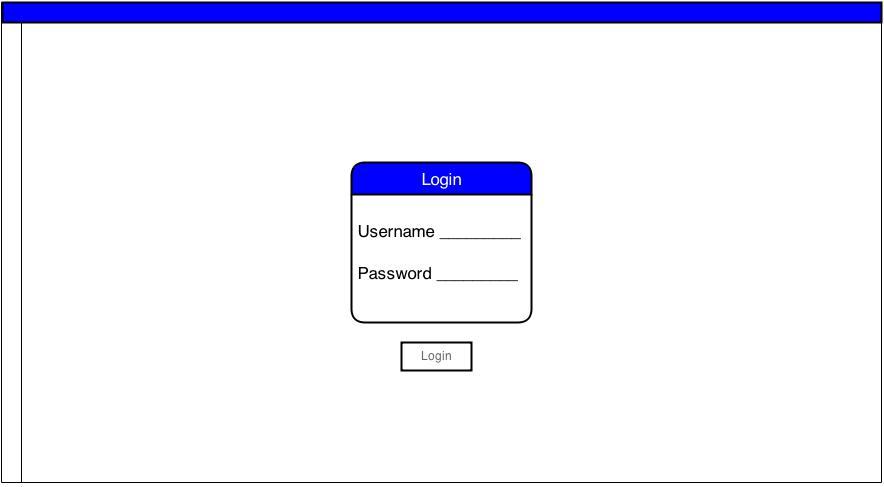
\includegraphics[height=7cm]{UILogin.jpg}}
            \caption{Login UI}
    \end{figure}
    \end{section}



%%%%%%%%%%%%%%%%%%%%%%%%%%%%%%%%%%%%%%%%%%%%%%%%%%%%%%%%%%%%%%%%%%%%%%%%%%%%%%%5
    \begin{section}{Student or instructor correctly logs out of the system}
        Description: The student or instructor is able to successfully log out of the system.\\
        Primary Actors: Student, Instructor\\
        Secondary Actor: System\\
        Steps:
        \begin{itemize}
            \item The student or instructor clicks the ''Log Out'' button.
            \item Successful Post Condition:
            \item The student or instructor receives a reply from the system that says that the log out was successful.
        \end{itemize}
        Exceptional Condition:
        \begin{itemize}
            \item The ''Logout'' button does not have the functionality to successfully log out the student or instructor.
        \end{itemize}


    \end{section}




%%%%%%%%%%%%%%%%%%%%%%%%%%%%%%%%%%%%%%%%%%%%%%%%%%%%%%%%%%%%%%%%%%%%%%%%%%%%%%%%%%%%%%%%%%%%
%%%%%%%%%%%%%%%%%%%%%%%%%%%%%%%%%%%%%%%%%%%%%%%%%%%%%%%%%%%%%%%%%%%%%%%%%%%%%%%%%%%%%%%%%%%%



\chapter{Professor UI Requirements}

    \begin{section}{Professor Clicks on Side or Top Navigation Buttons}
        Description: While on any page containing navigation links in the side or top bars, the professor clicks on a nav link \newline
        Primary Actors: Professor \newline
        Steps:
        \begin{enumerate}
            \item{The professor is logged into any of the main pages containing nav links}
            \item{The professor clicks on any link}
        \end{enumerate}
        Successful Post Conditions:
        \begin{itemize}
          \item{The professor is directed to the page intended by the link}
        \end{itemize}
        Exceptional Condition:
        \begin{itemize}
           \item{The professor is already on the page of the link they are clicking - nothing happens and the page does not change.}
        \end{itemize}
    \end{section}
    
    \begin{section}{Professor Clicks on the Assignment Submission Ticker}
        Description: From the main landing page the professor clicks on the assignment submission ticker \newline 
        Primary Actor: Professor \newline
        Steps:
        \begin{enumerate}
            \item{The professor is on the main page after login}
            \item{The professor clicks on the Assignment Submission Ticker Pane}
        \end{enumerate}
        Successful Post Condition:
        \begin{itemize}
            \item{The professor is redirected to a larger detailed view with a time directed log of student submission stats for assignments the professor has created, or is linked to through class ownership}
        \end{itemize}
        Exceptional Post Condition:
        \begin{itemize}
            \item{The professor has no submissions in his feed - he is directed to the log but is not shown any information}
        \end{itemize}
    \end{section}
    
    \begin{section}{Professor Clicks on the Class or Student Ticker}
        Description: From the main landing page the professor clicks on enrolled student/ class ticker pane \newline
        Primary Actor: Professor \newline
        Steps:
        \begin{enumerate}
            \item{The professor is on the main page after login}
            \item{The professor clicks on the enrolled student/ class ticker pane}
        \end{enumerate}
        Successful Post Condition:
        \begin{itemize}
            \item The professor is redirected to a larger detailed view with the option to sort by class or student name to display stats pertaining to course enrollment and individual student assignment histories
        \end{itemize}
    \end{section}
    
    \begin{section}{Professor Clicks to Expand the Assignment Creation Sandbox}
        Primary Actor: Professor \newline
        Steps:
        \begin{enumerate}
        \item{The professor is on the main page after login} 
        \item{The professor clicks to expand the assignment creation sandbox}
        \end{enumerate}
        Successful Post Condition:
        \begin{itemize}
        \item{The professor is taken to the assignment creation page and any potential diagrams or questions created in the sandbox are stored and transferred to the assignment creation window}
        \end{itemize}
    \end{section}
    
    \newpage
    \iffalse
    \begin{section}{Professor View}
        \begin{figure}[h!]
                \centerline{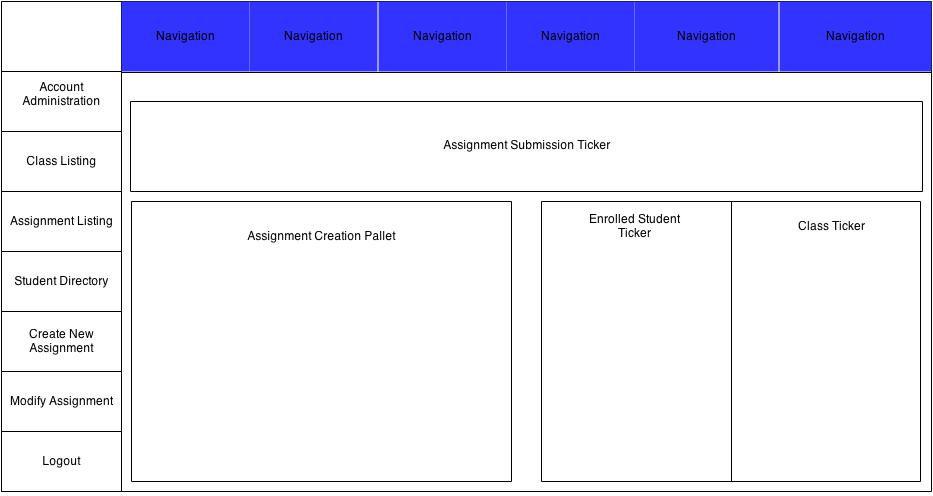
\includegraphics[width=13cm]{ProfessorView.jpg}}
                \caption{Professor's User Interface}
        \end{figure}
    \end{section}
    \newpage

    \begin{section}{Create}
        \begin{figure}[h!]
                \centerline{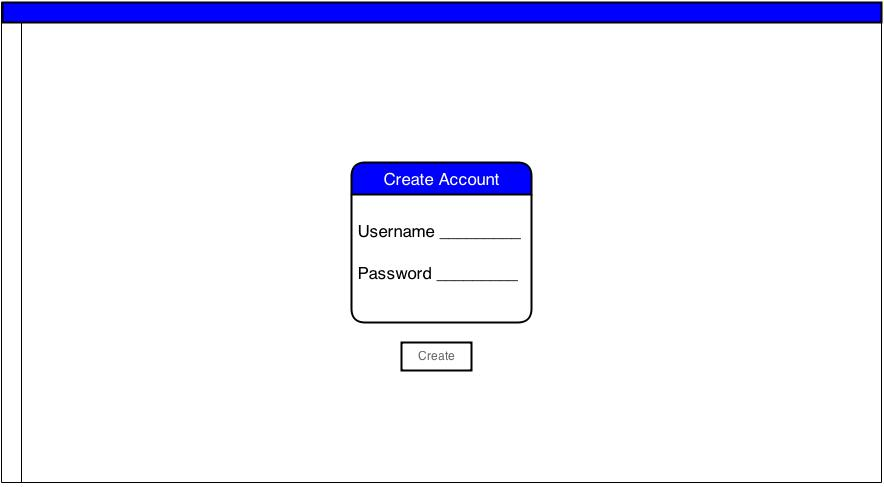
\includegraphics[width=13cm]{UICreate.jpg}}
                \caption{User Interface to create question}
        \end{figure}
    \end{section}
    \newpage
    \begin{section}{Login}
        \begin{figure}[h!]
                \centerline{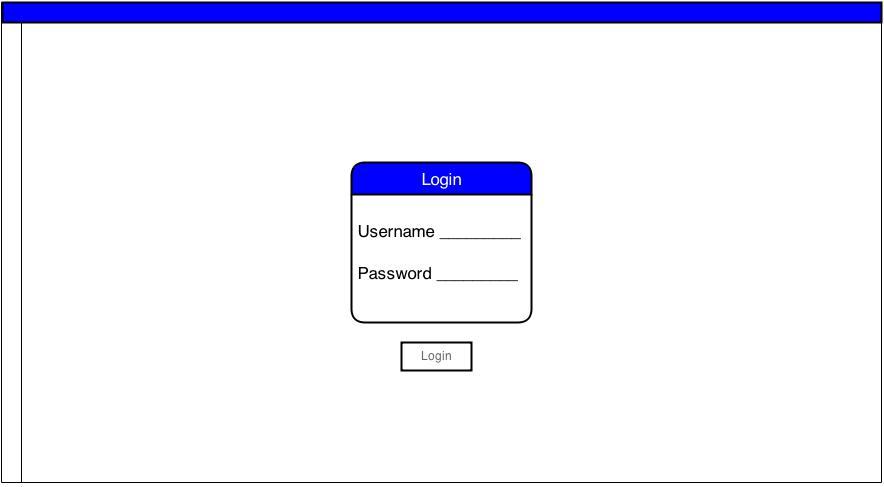
\includegraphics[width=13cm]{UILogin.jpg}}
                \caption{Login User Interface}
        \end{figure}
        \end{section}
        \newpage
        \begin{section}{Student}
        \begin{figure}[h!]
                \centerline{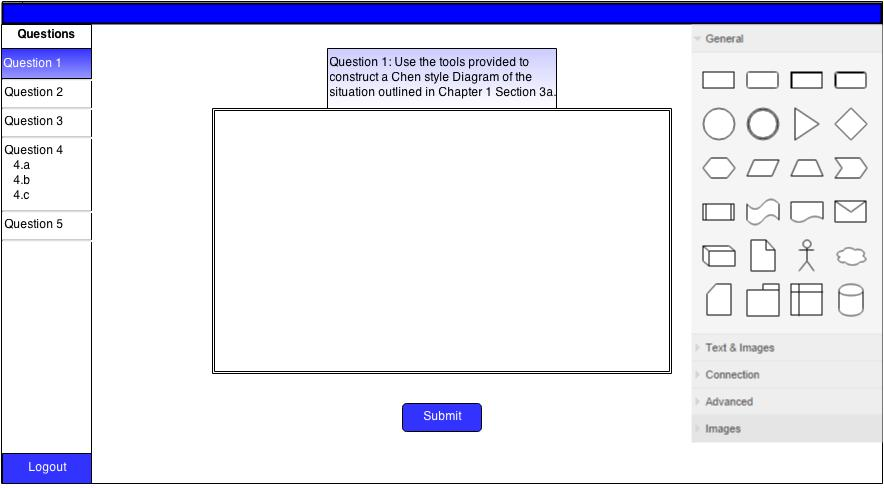
\includegraphics[width=13cm]{uistudent.jpg}}
                \caption{User Interface for the student}
        \end{figure}
  
    \end{section}

      \fi





















\end{document}

